\begin{hcarentry}{Blank Canvas}
\label{BlankCanvas}
\report{Andy Gill}%05/15
\participants{Justin Dawson, Andy Gill, Mark Grebe, Ryan Scott, James Stanton, Jeffrey Rosenbluth, and Neil Sculthorpe}
\status{active}
\makeheader

Blank Canvas is a Haskell binding to the complete HTML5 Canvas API.
Blank Canvas allows Haskell users to write, in Haskell, interactive images
onto their web browsers. Blank Canvas gives the user a single full-window
canvas, and provides many well-documented functions for rendering images.
Out of the box,
Blank Canvas is pac-man complete -- it is a platform
for simple graphics, classic video games,
and building more powerful abstractions that use graphics.

Blank Canvas was written in Spring 2012, as part of the
preparation for a graduate-level
functional programming class. 
In Fall 2012 and Fall 2013, we used Blank Canvas to teach Functional Reactive Programming.
This was our first hint that the Blank Canvas library was faster than we expected,
as we had hundreds of balls bouncing smoothly on the screen, much to the students' delight. 

Blank Canvas has now been used by the students in four separate
instances of our functional programming class. Students find it easy
to understand, given the analog between the IO monad, and the remote
Canvas monad,
%
with student often choosing to use Blank Canvas for their end-of-semester project. 
To give two examples,
one end-of-semester project was
%
Omar Bari and Dain Vermaak's Isometric Tile Game, that can 
be rotated in 3D in real-time;
%
another project was Blankeroids, a playable asteroids clone,
written by Mark Grebe, on top of Yampa and yampa-canvas.
%

%**<img width=200 src="./Isometric_Omar_Bari.png">
%*ignore
\begin{center}
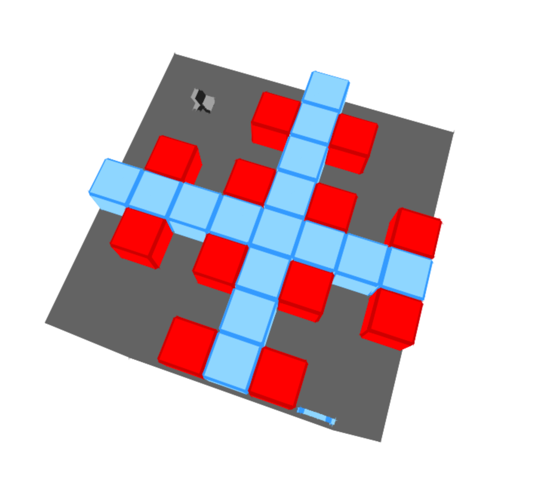
\includegraphics[width=0.235\textwidth]{html/Isometric_Omar_Bari.png}
\end{center}
%*endignore

%**<img width=200 src="./Isometric_Omar_Bari.png">
%*ignore
\begin{center}
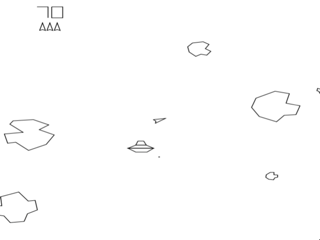
\includegraphics[width=0.235\textwidth]{html/Blankeroids_Mark_Grebe.png}
\end{center}
%*endignore

For more details, read the blank-canvas wiki.

\FurtherReading
\begin{compactitem}
\item
  \url{https://hackage.haskell.org/package/blank-canvas}
\item
  \url{https://github.com/ku-fpg/blank-canvas}
\item
  \url{https://github.com/ku-fpg/blank-canvas/wiki}
\end{compactitem}
\end{hcarentry}
